\chapter{Beeintr�chtigung des Wohlbefindens}
\section{Multitasking}

\paragraph*{}
Technische Ger�te wie Smartphones und Laptops sind ein fester Bestandteil der Gesellschaft geworden. Laut einer Studie \cite{Cyberkrank} im Jahr 2011 besa�en 96 \% von College-Studenten im Alter von 18 bis 22 Jahren ein Smartphone und 89\% Prozent 
f�r die bereits Arbeitenden im gleichen Alter.  In Deutschland kann man in den der gleichen Altersgruppe �hnliches vermerken. 2011 besitzen in Deutschland 25\% ein Smartphone, 2013 sind es bereits 72\% Prozent \cite{Cyberkrank}. Dies ist nun 5 Jahre her 
also kann man davon ausgehen, dass die �berwiegende Mehrheit heutzutage ein Smartphone besitzt.
\paragraph*{}
Digitale Medien, welche rund um die Uhr �ber das Smartphone in der Tasche leicht zu erreichen sind, regen zum Multitasking an. Dabei ist es schwierig  f�r Menschen Multitasking zu betreiben. Prof Dr. Torsten Schubert 
von der Humboldt\-Universit�t  behauptet dass Multitasking durch Entscheidungsprozesse zu einer erh�hten Fehlerquote oder einer verl�ngerten Bearbeitungszeit\cite{Gehirn}. 
\paragraph*{}
Gem�� Schubert gilt generell: Wenn Aufgaben das gleiche Hirnareal beanspruchen, st�ren sie sich und  dadurch wird Multitasking ineffizient. Die Natur des Menschen diktiert ihm sich vollst�ndig auf eine Aufgabe zu konzentrieren um diese zum Besten seiner 
F�higkeiten zu erledigen. Multitasking wird mit dem Antrainieren von Sucht und Aufmerksamkeitsst�rungen gleichgestellt\cite{Gehirn}.
\paragraph*{}
Jugendliche nutzen ihr Smartphone 150 Mal am Tag, folglich wird eine T�tigkeit im Durschnitt alle 6 Minuten unterbrochen \cite{iDisorder}. Die Psychologin Lydia Burak von der Bridgewater State University f�hrte  eine Umfrage, \cite{Cyberkrank} 
(Massachusetts, USA) die bei einer Testgruppe von 774 Studenten im Alter von 20 bis 75 Jahren und einer Verteilung der Geschlechter von 67,1\% weiblich und 32,9\% m�nnlich mittels Fragebogen feststellt, dass sich nur 5,6\% nicht noch mit anderen Aktivit�ten 
w�hrend der Lehrveranstaltungen besch�ftigen. Dies ist interessant, da mithilfe eines Multiple-Choice Test sofort nach einer Vorlesung, die den darin behandelten Stoff abfragt festgestellt werden konnte, dass die abgelenkten Studenten (Multitasking) 
schlechtere Resultate erzielten \cite{Cyberkrank}.

\begin{figure}
\centering
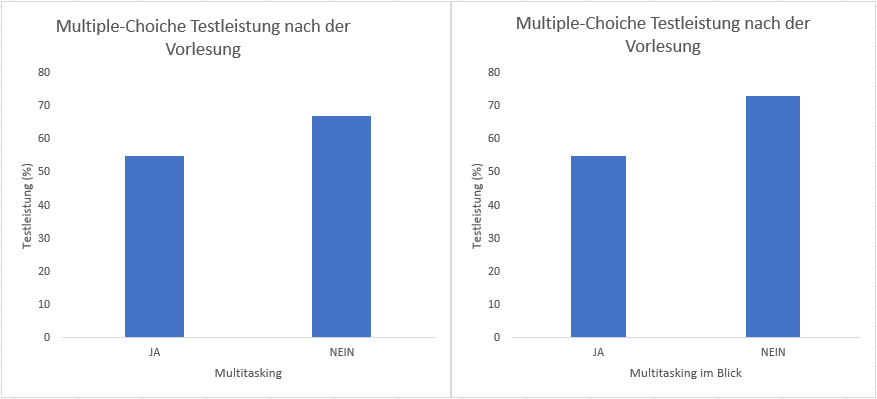
\includegraphics[scale=0.635]{images/graphtest.png}
\caption{H�ufigkeit korrekter Antworten im Test nach der Vorlesung in Abh�ngigkeit davon, ob die Studenten zugleich mit anderen Aufgaben am Computer selbst besch�ftigt waren oder nicht (linke Abbildung) bzw. davon, ob die Studenten anderen Studenten beim Multitasken am Laptop zuschauen konnten oder nicht (rechte Abbildung).}
\end{figure}

\break

\section{Tr�bung der menschlichen Psyche}
\paragraph*{}
Das Verwenden von Smartphones und Laptops st�rt das Lernen direkt durch Konzentrationsverlust w�hrend Lehrveranstaltungen und beeinflussen indirekt die akademische Leistung.
\paragraph*{}
Eine Studie in Schweden von Biomedcentral Public Health \cite{Mobile} konnte  im Jahr 2011 mit 4156 Probanden aus der schwedischen Bev�lkerung, davon 1455 m�nnlich und 2701 weiblich, eine Relation erstens zwischen hohem Mobiltelefongebrauch und Stressempfinden, und zweitens zwischen Schlafst�rungen und Symptomen von Depression feststellen. Die Probanden sind in einem Alter von 20 -24 Jahren von welchen 40\% der M�nner und 48\% der Frauen studieren.  Eine weiter Studie in Schweden von Biomedcentral Psychiatrics \cite{Computer} im Jahr 2012 mit 4163 Probanden im gleichen Alter, davon 1458 m�nnlich und 2705 weiblich, untersucht die gleichen Folgen bei hohem Computergebrauch .
\paragraph*{}
Beide Studien verbinden die verbrachte Menge an Zeit mit Mobiletelefone also die Konstante Erreichbarkeit oder vor dem Computer mit entweder einem Risiko f�r erh�htes Stressempfinden, Schlafst�rungen oder Entwicklung von Symptomen der Depression.
\paragraph*{}
Desto mehr Zeit vor einem Bildschirm verbracht wird desto gr��er ist auch der Einfluss auf die Art wie der Mensch mit seinem Sozialen Umfeld interagiert. In Neuseeland im Rahmen einer Studie \cite{Adolescent} von PhD. Rosalina Richards, PhD Rob McGee, D.Sc Sheila M. Williams, PhD. David Welch and MD Robert J. Hancox wurden 1987\-1988, 976 Jugendliche im Alter von 15 Jahren befragt wieviel Zeit sie vor dem Fernseher verbringen und es wurde ihre Beziehung zu Gleichaltrigen und ihren Eltern bewertet mittels einer gek�rzten Version von \"Inventory of Parent and Peer Attachment\"(IPPA).
\paragraph*{}
In der gleichen Studie wurden 2004 3983 Sch�ller aus 144 verschiedenen Schulen die gleichen Fragen gestellt und als Erg�nzung wurden die Probanden gefragt wieviel Zeit sie vor dem Computer verbringen, wieviel Zeit sie mit Lesen und dem erledigen von Hausaufgaben in ihrer Freizeit verbringen.
\paragraph*{}
In der ersten Phase 1987-1988 konnte man feststellen, dass jeder weiter Stunde vor dem Fernseher das Risiko eine schlechte Beziehung mit den Eltern zu haben um 13\% erh�ht und mit Gleichaltrigen sogar um 24\%. In der zweiten Phase 2004 war das Resultat �hnlich, mehr Zeit vor dem Bildschirm egal ob Fernseher oder Computer f�hrte zu einem h�heren Risiko eine schlechte Beziehung zu den Eltern oder Gleichaltrigen zu f�hren. Zeit mit Lesen und der Bew�ltigung von Hausaufgaben wurde hingegen mit einer besseren Beziehung zu den Eltern in Zusammenhang gebracht.
